\chapter{Resultados}\label{cap:resultados}

\section{Interface Gráfica}\label{sec:gui}

\FloatBarrier

\begin{figure}[h]
  \centering
  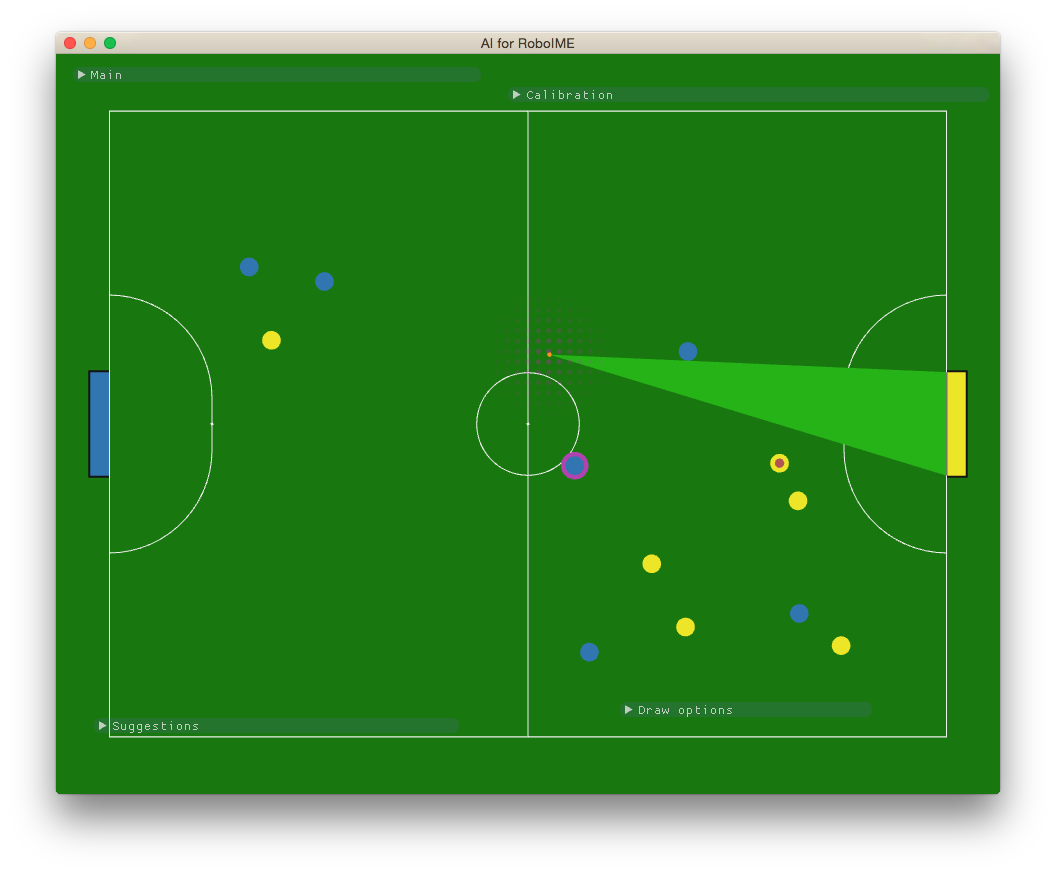
\includegraphics[width=0.8\linewidth]{gui_field}
  \caption{Aparência geral e representação do campo}\label{fig:gui_field}
\end{figure}

A ferramenta representa o estado atual do jogo desenhando o campo, os robôs e a
bola, como pode ser visto na Figura~\ref{fig:gui_field}.  O campo não faz parte
do estado mas é necessário para ter uma referência visual das posições.

\begin{figure}[h]
  \centering
  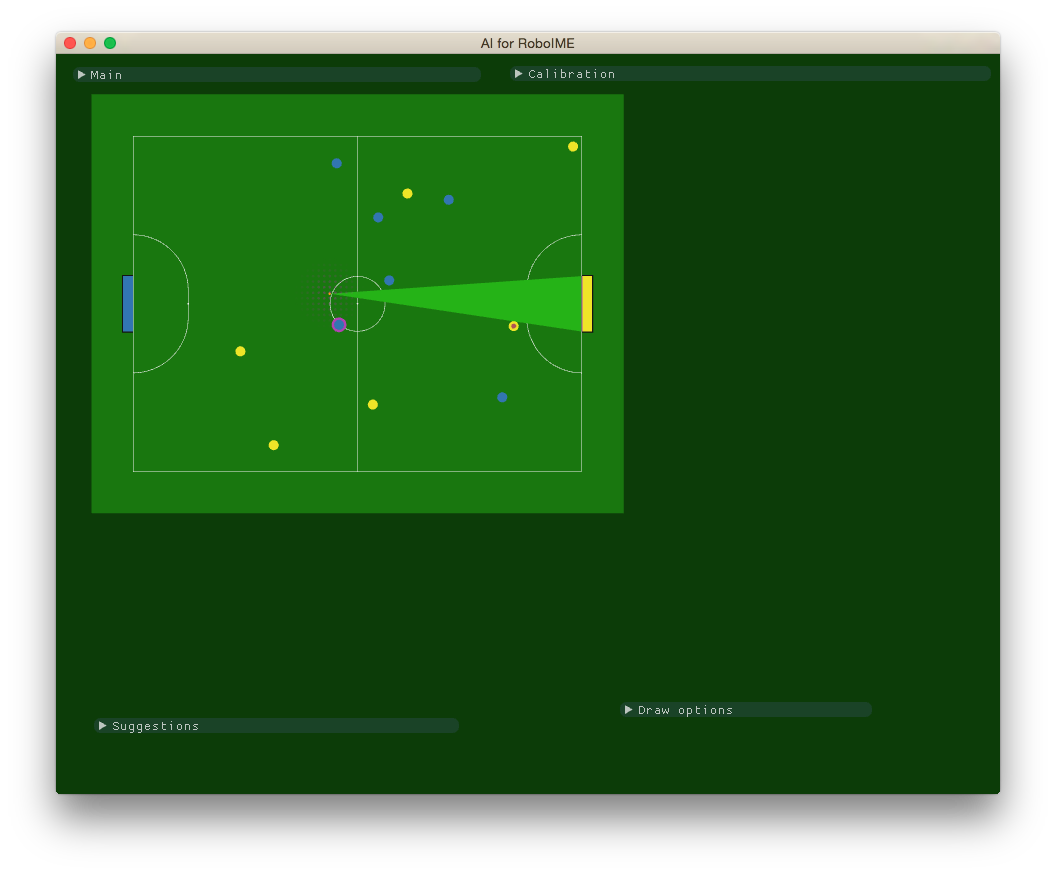
\includegraphics[width=0.4\linewidth]{gui_zoom_out}
  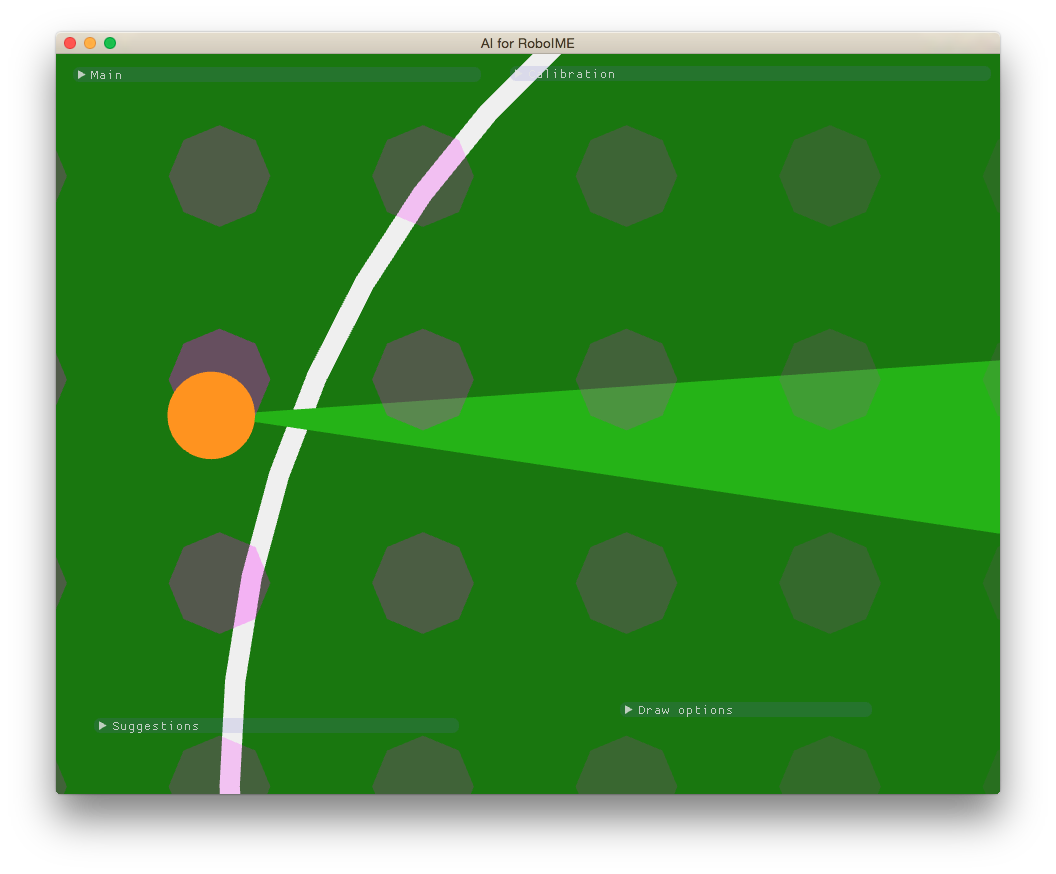
\includegraphics[width=0.4\linewidth]{gui_zoom_in}
  \caption{Zoom e arraste do campo}\label{fig:gui_zoom}
\end{figure}

Para visualizar situações com mais detalhes a ferramenta permite zoom e arraste
do campo (Figura~\ref{fig:gui_zoom}).

\FloatBarrier

\begin{figure}[h]
  \centering
  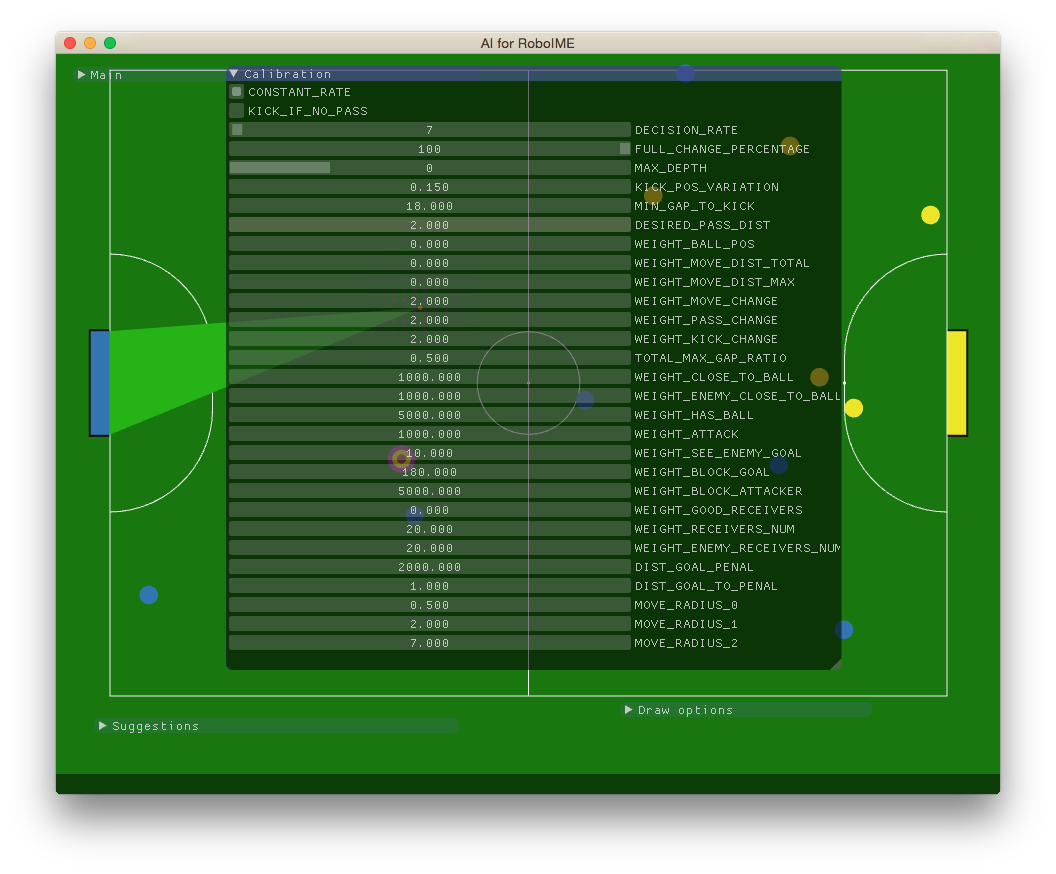
\includegraphics[width=0.75\linewidth]{gui_params}
  \caption{Parâmetros configuráveis}\label{fig:gui_params}
  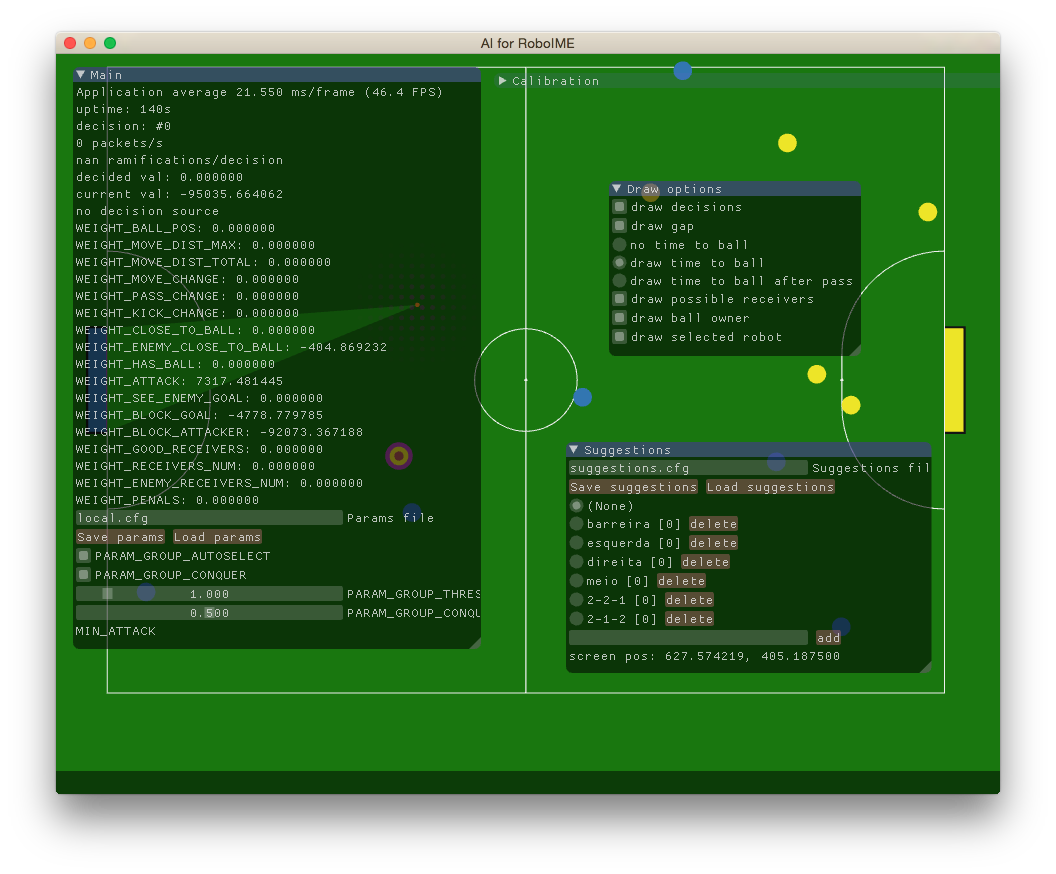
\includegraphics[width=0.75\linewidth]{gui_widgets}
  \caption{Controles}\label{fig:gui_widgets}
\end{figure}

\FloatBarrier

Existem quatro abas disponíveis: \textit{Main}, \textit{Calibration},
\textit{Suggestions}, \textit{Draw options}. As abas são retráteis e
translucidas para que as mudanças de configurações possam ser observadas
facilmente.  Na Figura~\ref{fig:gui_field}, por exemplo, todas as estão
minimizadas, na Figura~\ref{fig:gui_params} é mostrada a aba
\textit{Calibration}, as outras três podem ser vistas na
Figura~\ref{fig:gui_widgets}.

\begin{figure}[h]
  \centering
  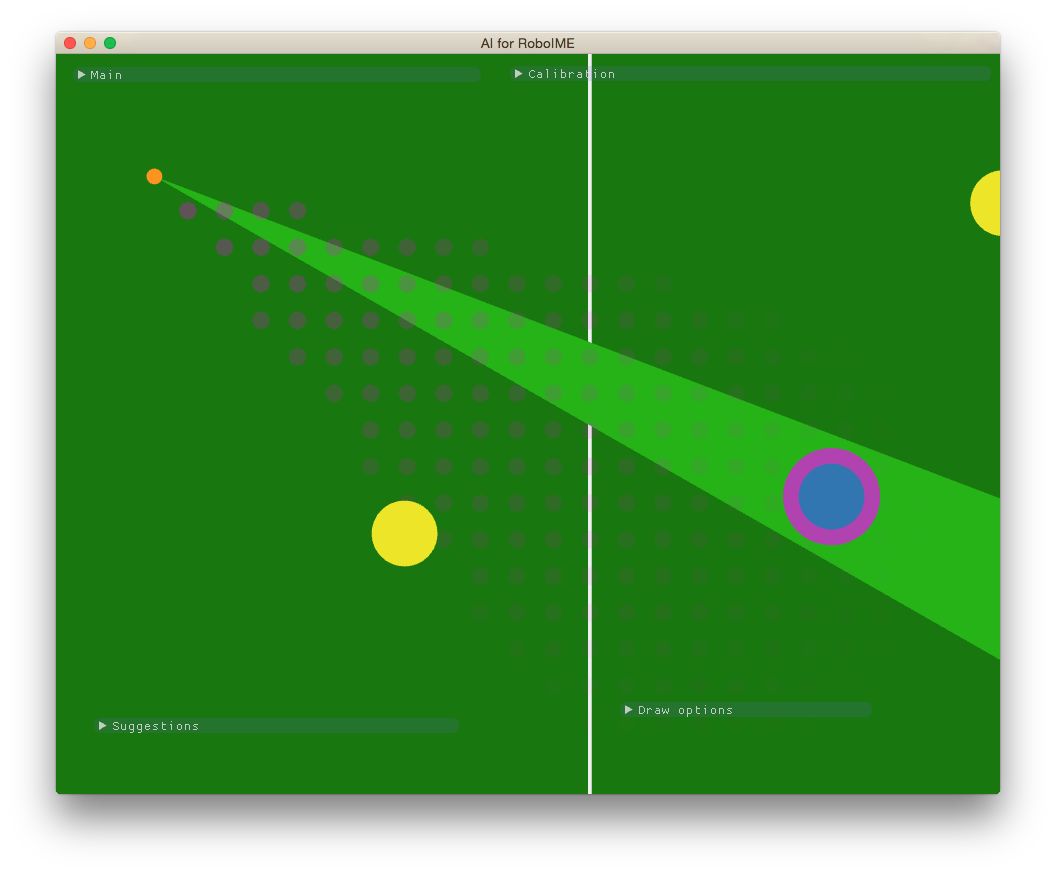
\includegraphics[width=0.4\linewidth]{gui_ball_move}
  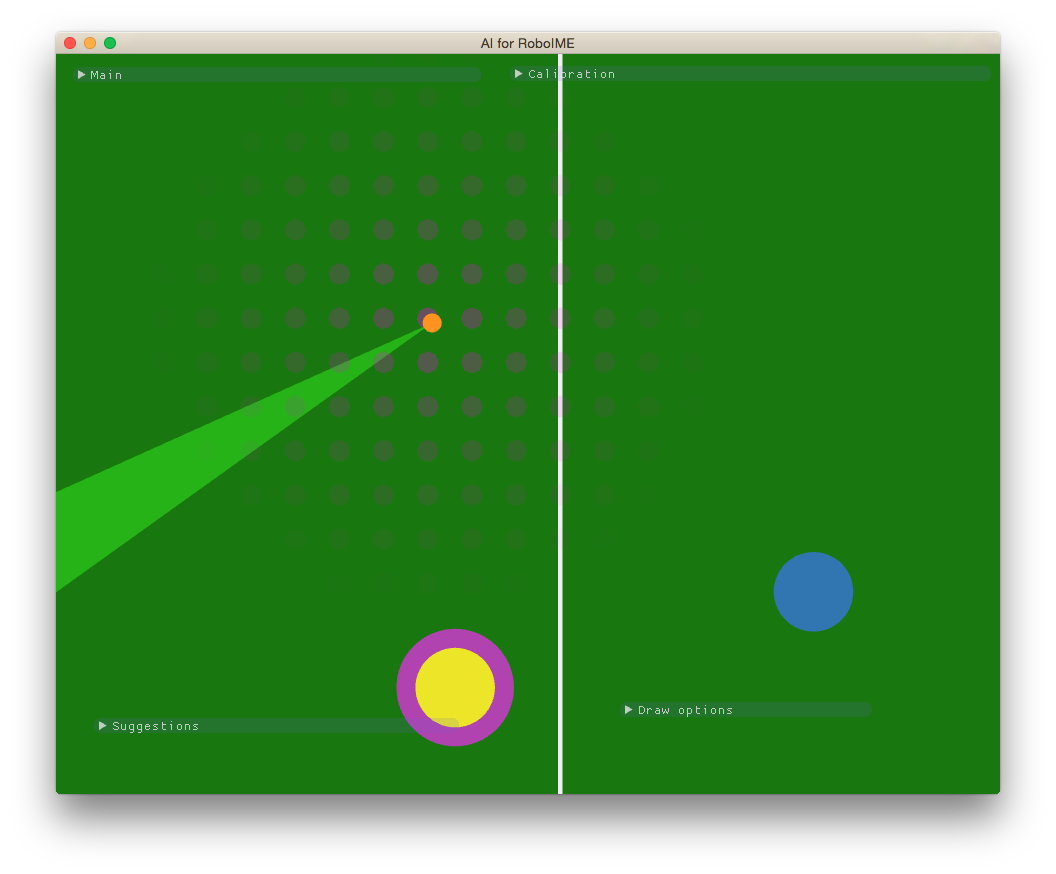
\includegraphics[width=0.4\linewidth]{gui_ball_stop}
  \caption{Representação do tempo para chegar na bola}\label{fig:gui_ball}
\end{figure}

A interface também possui indicadores para o tempo de chegar na bola, o robô que
chegará primeiro na bola e os robôs que podem receber um passe.

O indicador do robô que chegará primeiro, às vezes chamado de "dono da bola", é
representado com um círculo rosa em torno do robô.

O indicador para o tempo de chegar na bola está representado na
Figura~\ref{fig:gui_ball} como um campo de pontos translúcidos ao redor da bola,
quanto mais vizível o ponto menor o tempo para se chegar na bola a partir dali.
Na imagem à direita a bola está parada e o robô amarelo é o dono, já na imagem
da esquerda a bola está em movimento, aproximadamente na direção do robô azul,
que nesse caso é o dono da bola.


\begin{figure}[h]
  \centering
  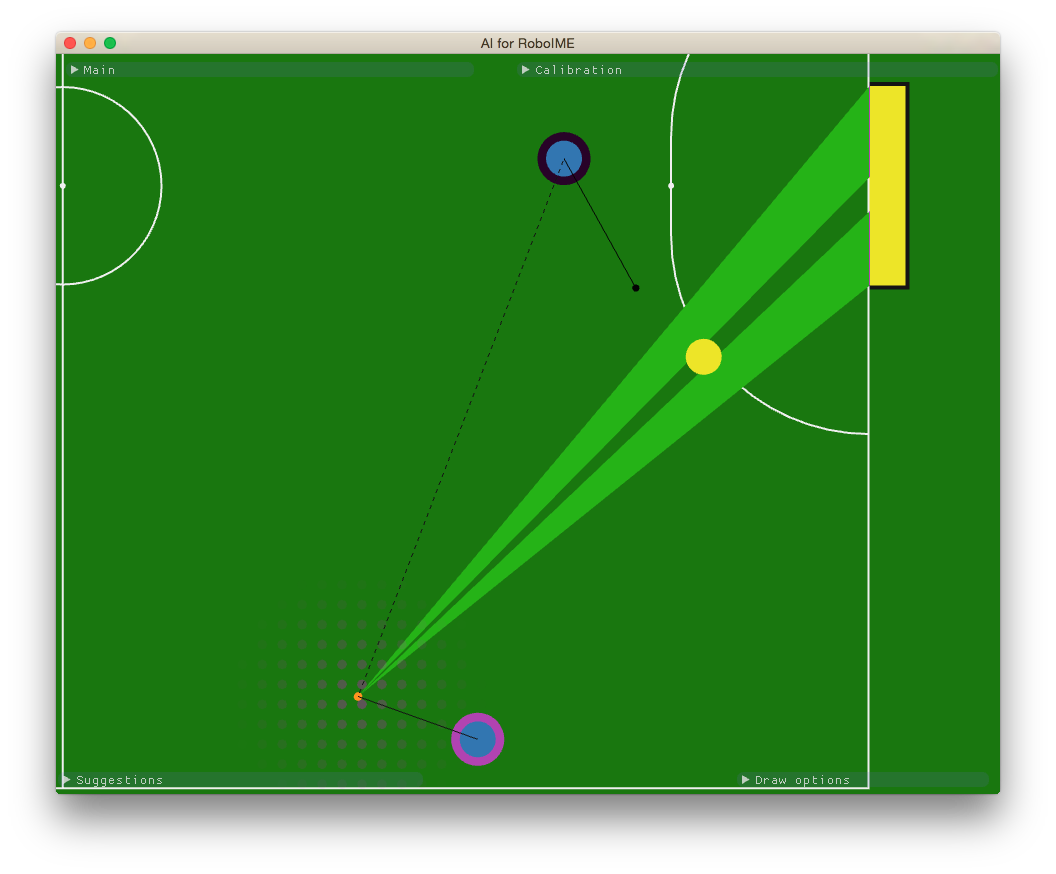
\includegraphics[width=0.8\linewidth]{gui_pass}
  \caption{Representação de ação de passe}\label{fig:gui_pass}
\end{figure}

\begin{figure}[h]
  \centering
  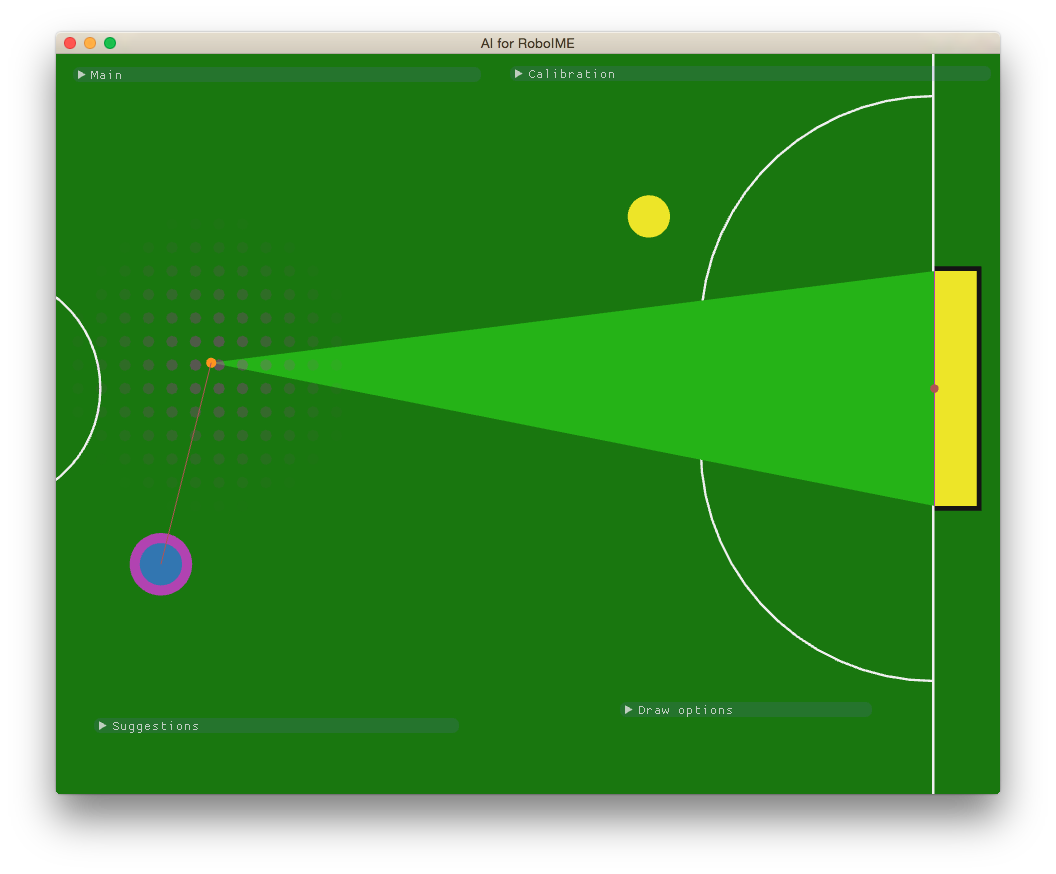
\includegraphics[width=0.8\linewidth]{gui_kick}
  \caption{Representação de ação de chute}\label{fig:gui_kick}
\end{figure}

\begin{figure}[h]
  \centering
  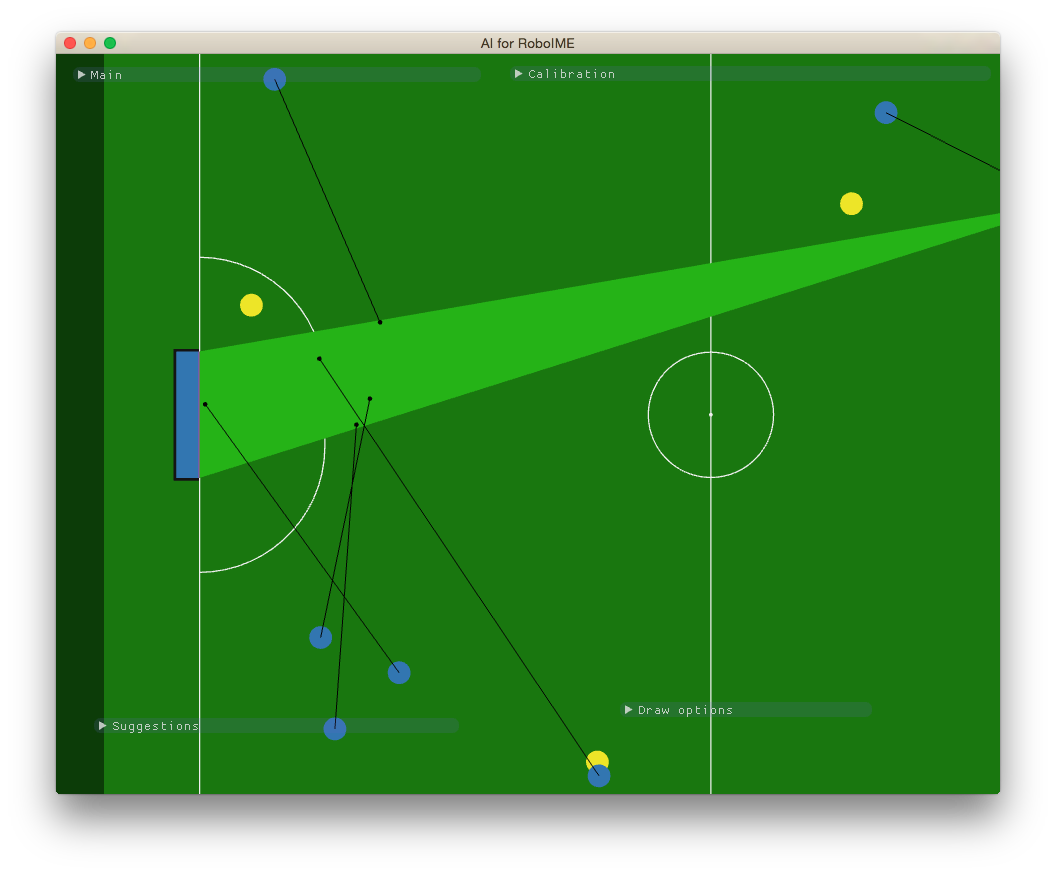
\includegraphics[width=0.8\linewidth]{gui_move}
  \caption{Representação das ações de movimentação}\label{fig:gui_move}
\end{figure}

As decisões tomadas possuem representação gráfica, desenhando individualmente
cada ação.  As ações de passe podem ser vistas na Figura~\ref{fig:gui_pass} uma
linha tracejada da bola para o receptor do passe, nessa mesma figura está
exemplificado a representação dos robôs que podem receber passe.

Similarmente a Figura~\ref{fig:gui_kick} apresenta a representação da ação de
chute.  E por fim, o último tipo de ação e mais comum, a de movimentação, pode
ser vista na Figura~\ref{fig:gui_move}.

\FloatBarrier

% vim: tw=80 et ts=2 sw=2 sts=2 ft=tex


\section{Influência dos Parâmetros no Comportamento do Time}

Nesta secção são apresentados os diferentes comportamentos
que podem ser obtidos através da modificação dos parâmetros
apresentados no capítulo~\ref{cap:modelagem}. Cada parâmetro
é modificado e os resultados na mudança do planejamento são
evidenciados.

Os parâmetros iniciais são definidos no arquivo src/consts.h, % TODO: referenciar anexos
cujos valores são:

% TODO: Substituir nomes das variáveis, conforme a modelagem
\begin{enumerate}
  \item $FULL{\_}CHANGE{\_}PERCENTAGE = 100$
  \item $KICK{\_}POS{\_}VARIATION = 0.150$
  \item $MIN{\_}GAP{\_}TO{\_}KICK = 18.0$
  \item $DESIRED{\_}PASS{\_}DIST = 2.0$
  \item $WEIGHT{\_}MOVE{\_}DIST{\_}MAX = 0$
  \item $WEIGHT{\_}MOVE{\_}DIST{\_}TOTAL = 0$
  \item $WEIGHT{\_}ATTACK = 1000$
  \item $WEIGHT{\_}SEE{\_}ENEMY{\_}GOAL = 10$
  \item $WEIGHT{\_}BLOCK{\_}GOAL = 180$
  \item $WEIGHT{\_}BLOCK{\_}ATTACKER = 5000$
\end{enumerate}

A figura~\ref{fig:default} apresenta o planejamento em um
ambiente de ataque e defesa com os parâmetros iniciais
apresentados anteriormente.

\begin{figure}[H]
  \centering
  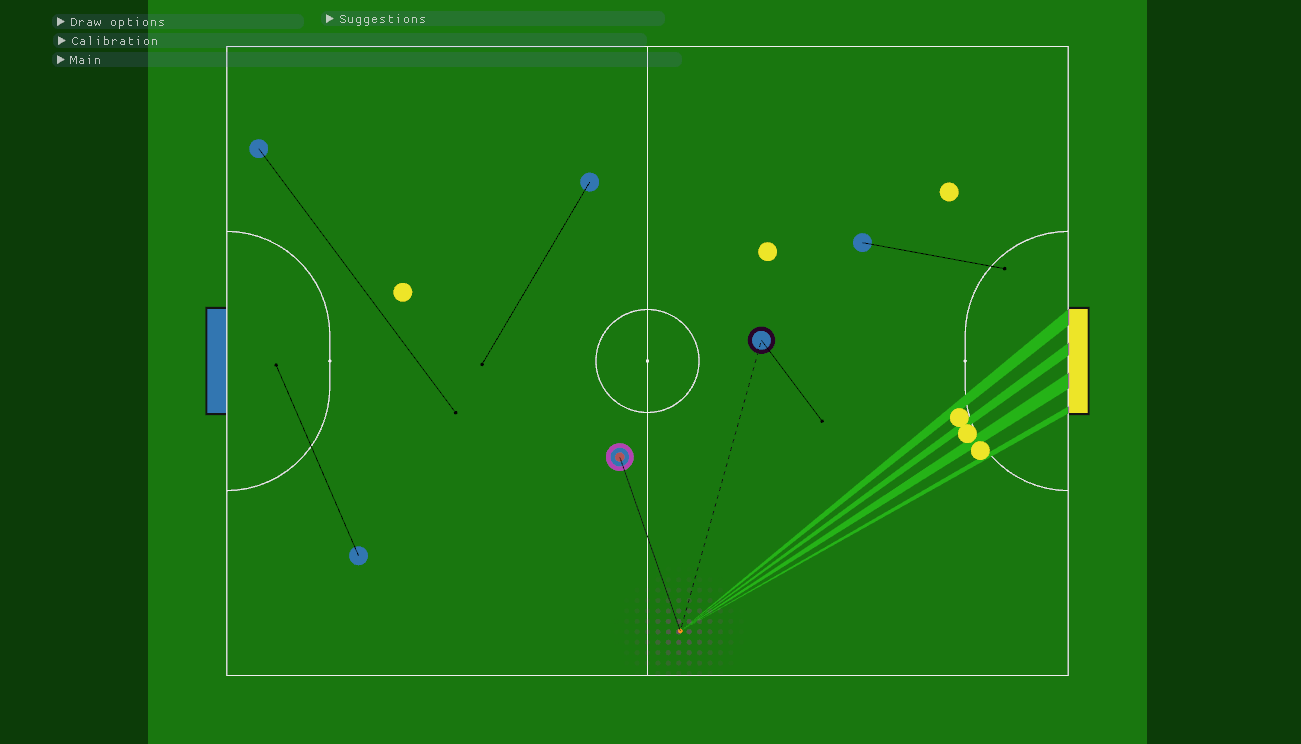
\includegraphics[width= 0.8\linewidth]{result/default_atq}
  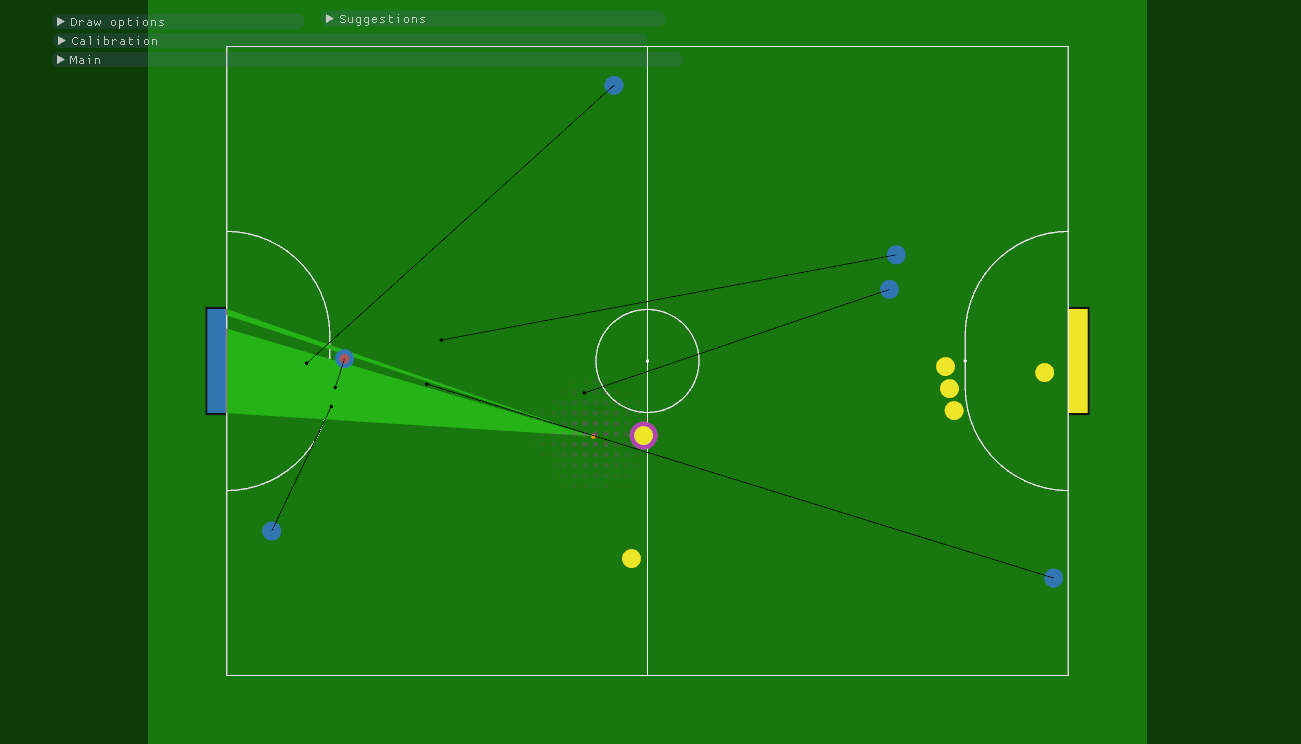
\includegraphics[width= 0.8\linewidth]{result/default_def}
  \caption{Planejamento com os parâmetros iniciais no
           ataque (acima) e na defesa (abaixo)}\label{fig:default}
\end{figure}

\subsection{Correção da Abertura do Gol Devido a Movimentação da Bola}

Somente o ajuste de movimentação da bola foi anulado. Os resultados
no planejamento são apresentados na Figura~\ref{fig:kickpos_0}.
Conforme pode ser observado, a sombra dos robôs é maior, reduzindo
assim abertura do gol. Logo, poucos robôs são necessários
para bloquear o gol. Isso gerou mais ações direcionadas para posições
de ataque.

\begin{figure}[H]
  \centering
  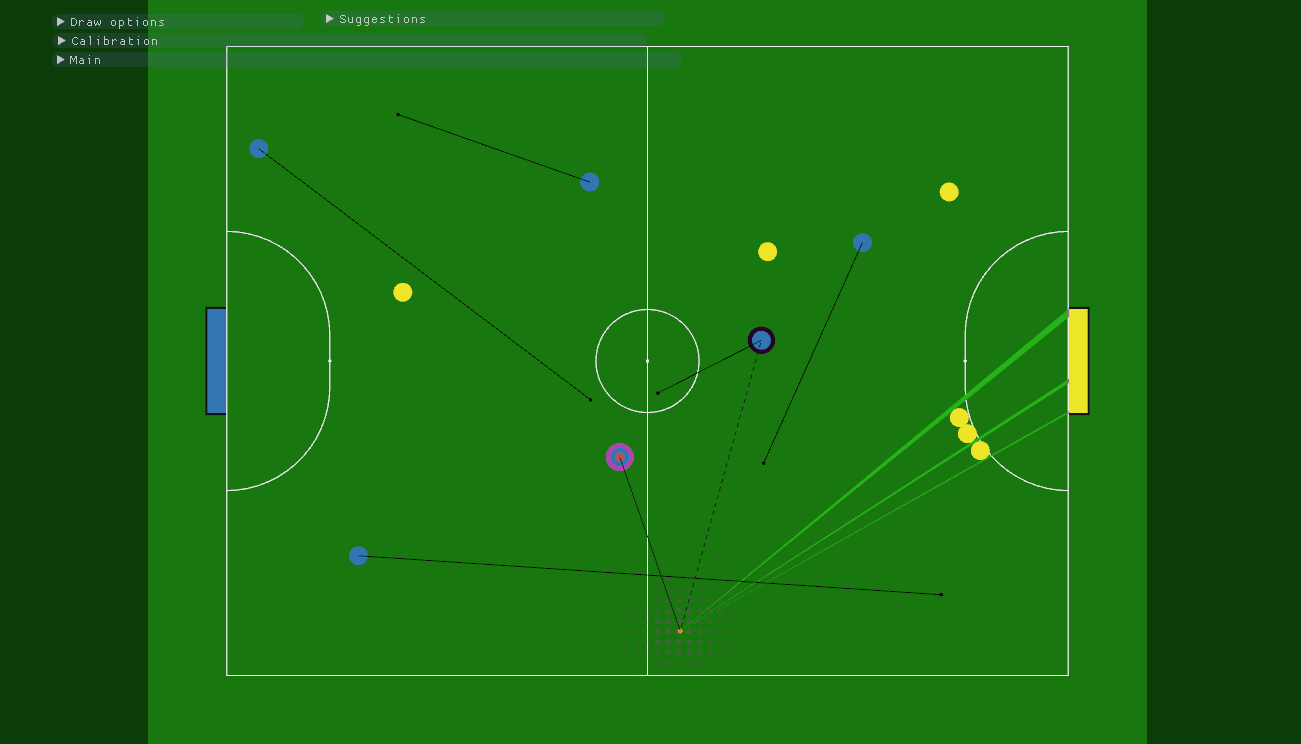
\includegraphics[width= 0.8\linewidth]{result/kickpos_0_atq}
  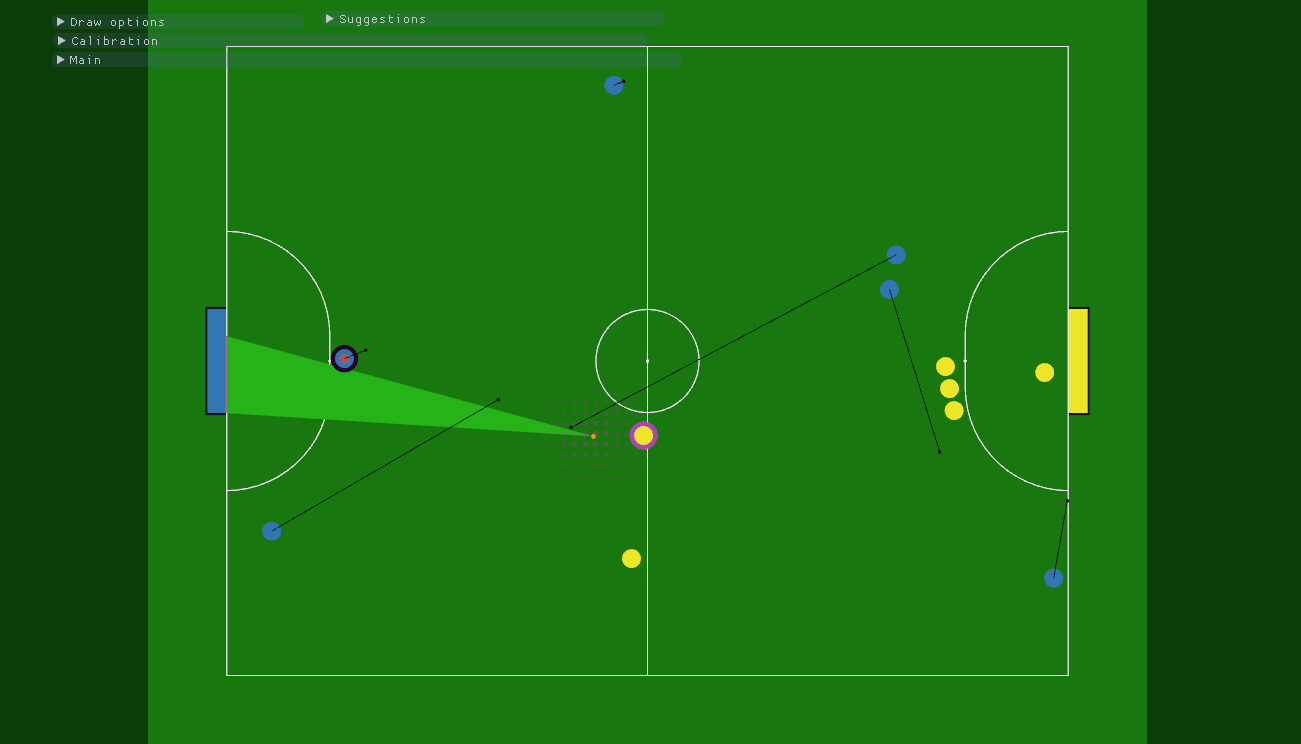
\includegraphics[width= 0.8\linewidth]{result/kickpos_0_def}
  \caption{Planejamento com os parâmetros inicias e sem ajuste
           de movimentação da bola em ambiente de
           ataque (acima) e defesa (abaixo)}\label{fig:kickpos_0}
\end{figure}

Depois esse ajuste foi alterado para $0.24$. Os resultados 
em ambiente de ataque e defesa são apresentados na
Figura~\ref{fig:kickpos_024}. A sombra de cada robô é
menor, resultando em mais robôs próximos ao gol para
reduzir a abertura do gol vista pelos robôs adversários.

\begin{figure}[H]
  \centering
  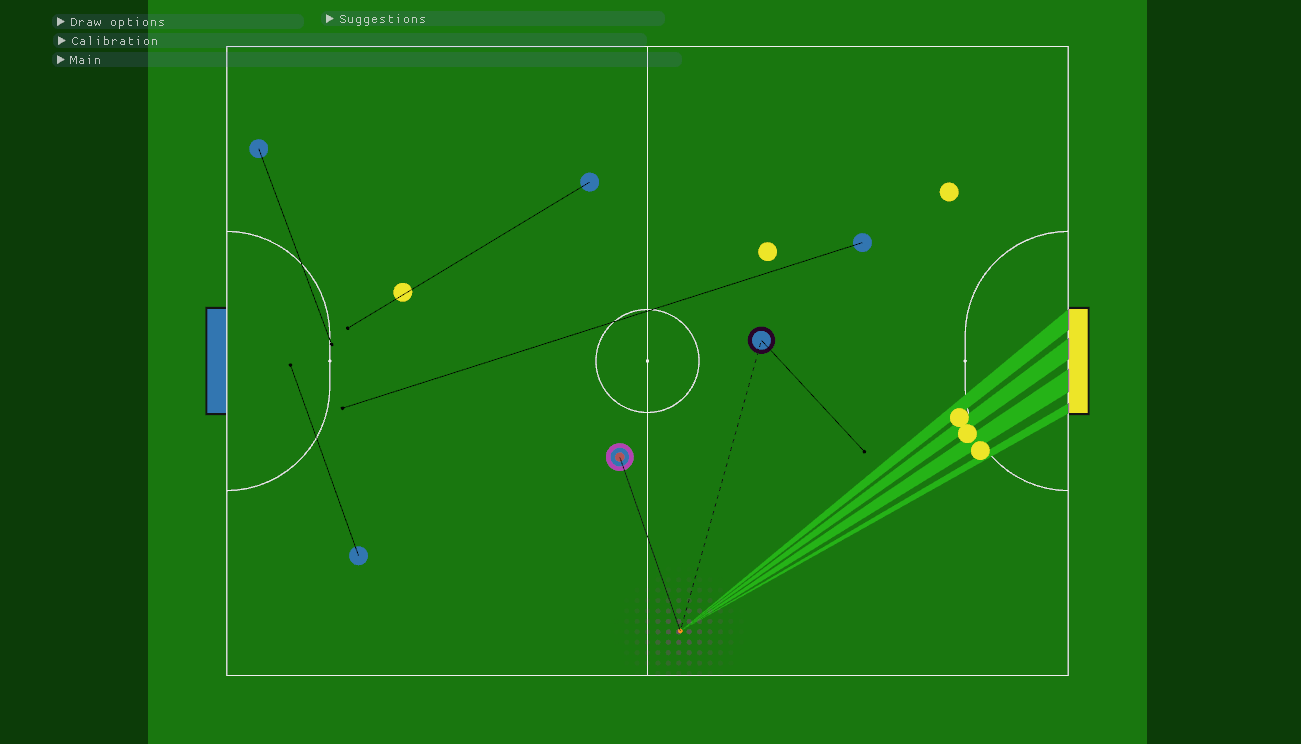
\includegraphics[width= 0.8\linewidth]{result/kickpos_024_atq}
  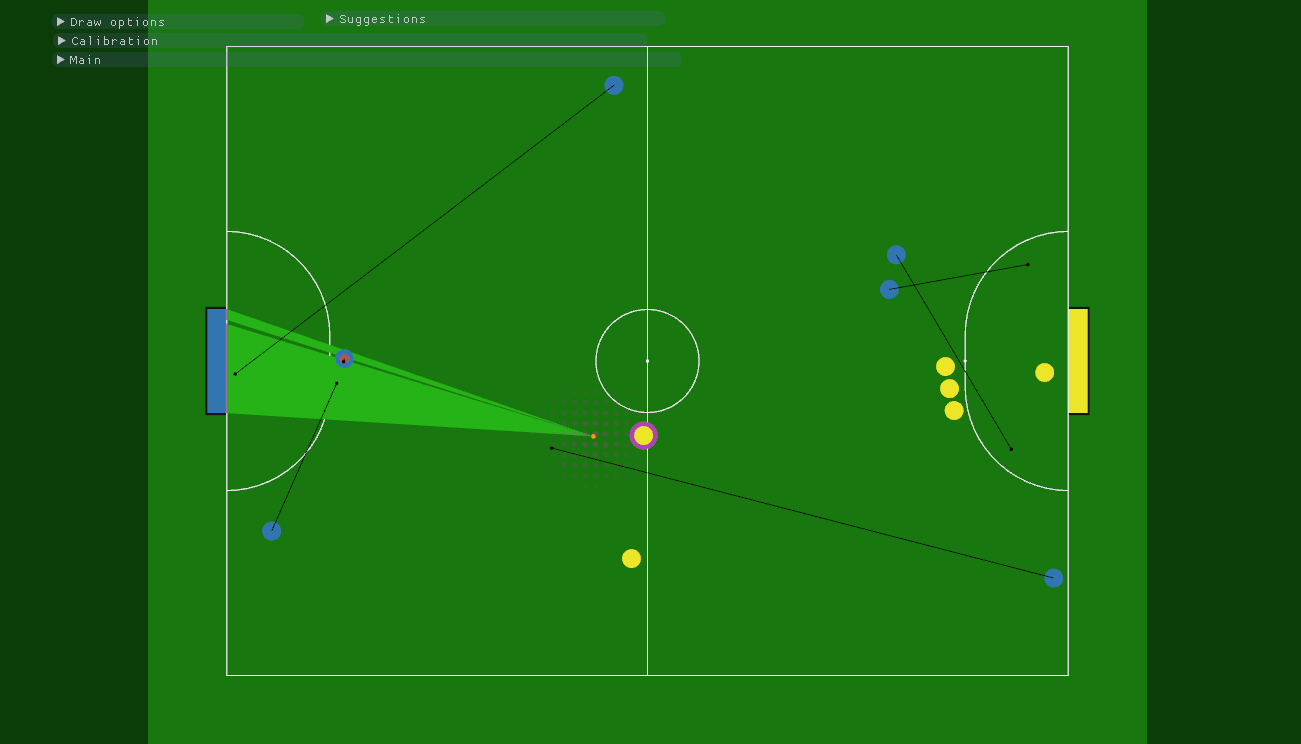
\includegraphics[width= 0.8\linewidth]{result/kickpos_024_def}
  \caption{Planejamento com os parâmetros inicias e o ajuste de
           movimentação da bola ajustado para $0.24$ em ambiente de
           ataque (acima) e defesa (abaixo)}\label{fig:kickpos_024}
\end{figure}

\subsection{Distância Total dos Moves}

Somente o peso do custo da distância total dos moves foi alterado para $10$. Os
resultados no planejamento são apresentados na
Figura~\ref{fig:mov_dist_total_10}.

\begin{figure}[H]
  \centering
  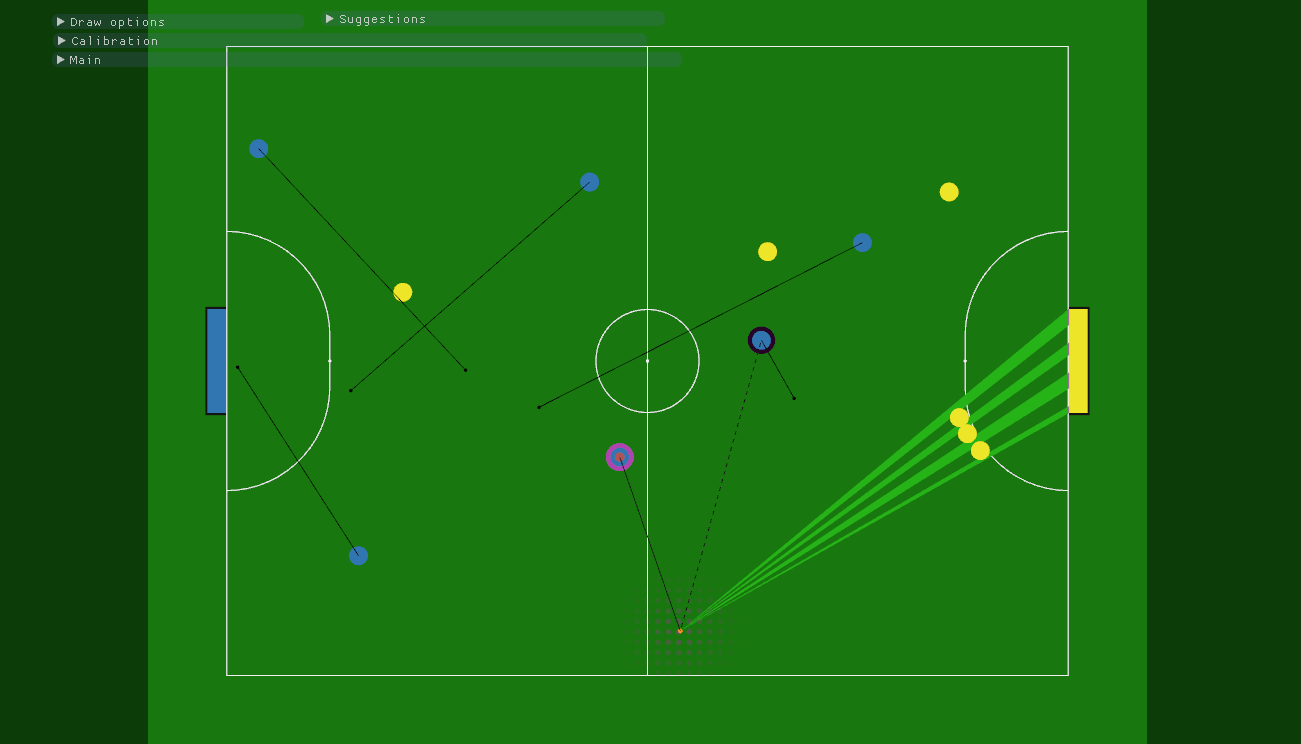
\includegraphics[width= 0.8\linewidth]{result/mov_dist_total_atq_10}
  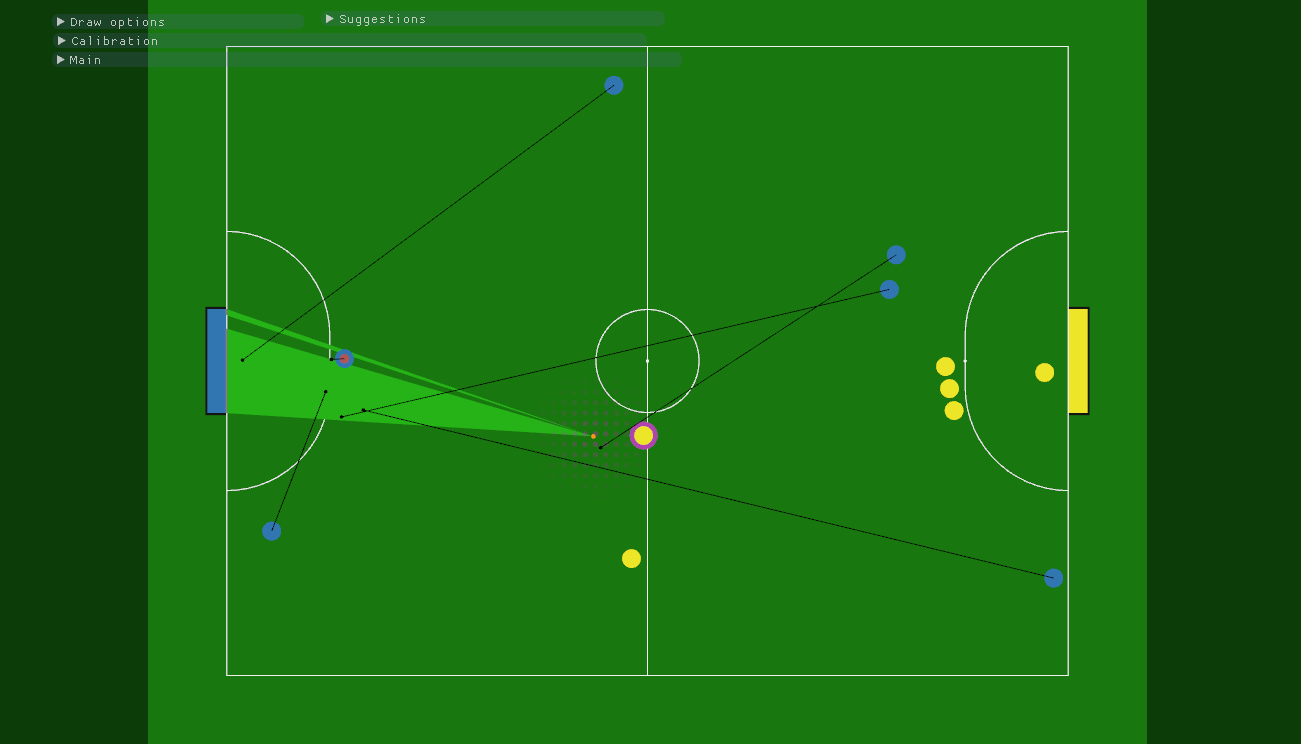
\includegraphics[width= 0.8\linewidth]{result/mov_dist_total_def_10}
  \caption{Planejamento com os parâmetros iniciais e o peso do custo da
  distância total dos moves alterado para $10$.  Ataque (acima) e na defesa (abaixo)}\label{fig:mov_dist_total_10}
\end{figure}

% vim: tw=80 et ts=2 sw=2 sts=2 ft=tex

\subsection{Distância Máxima dos Moves} 
Somente o peso do custo da distância máxima dos moves foi
alterado para $10$. Os resultados no planejamento são
apresentados na figura~\ref{fig:mov_dist_max_10}.

\begin{figure}[H]
  \centering
  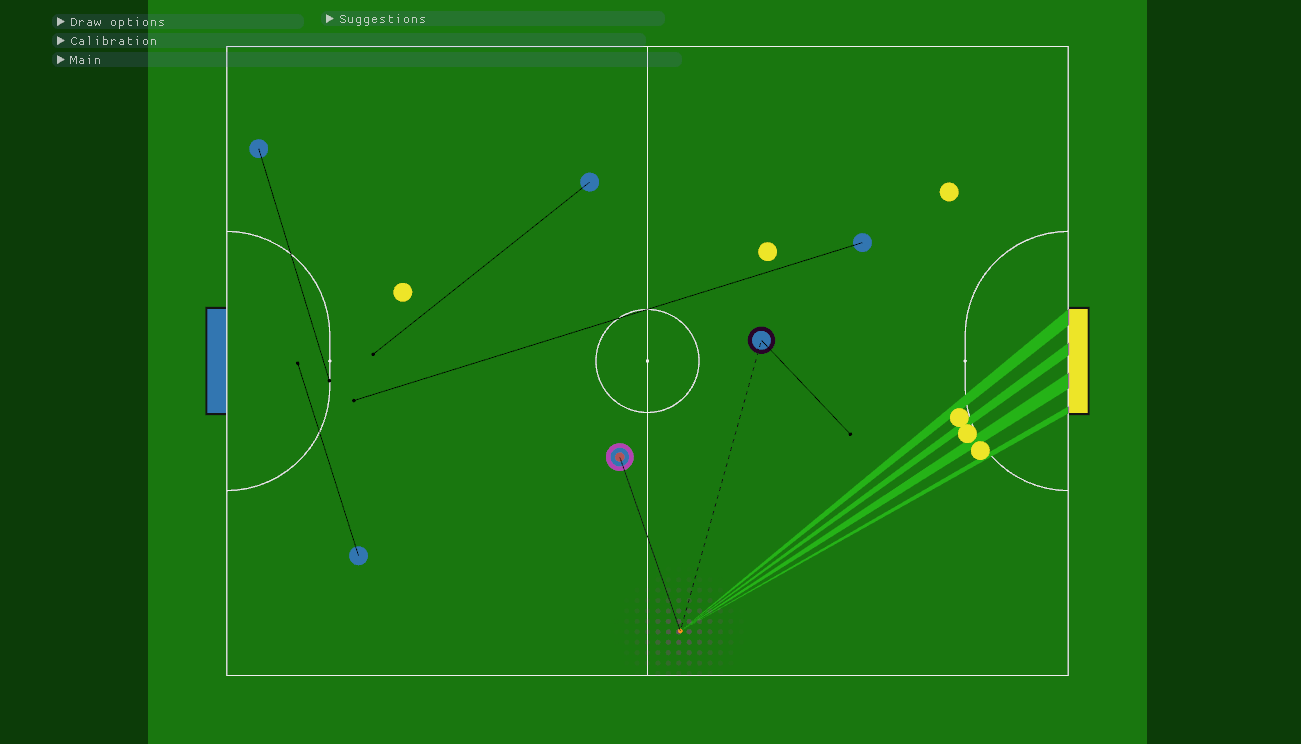
\includegraphics[width= 0.8\linewidth]{result/mov_dist_max_atq_10}
  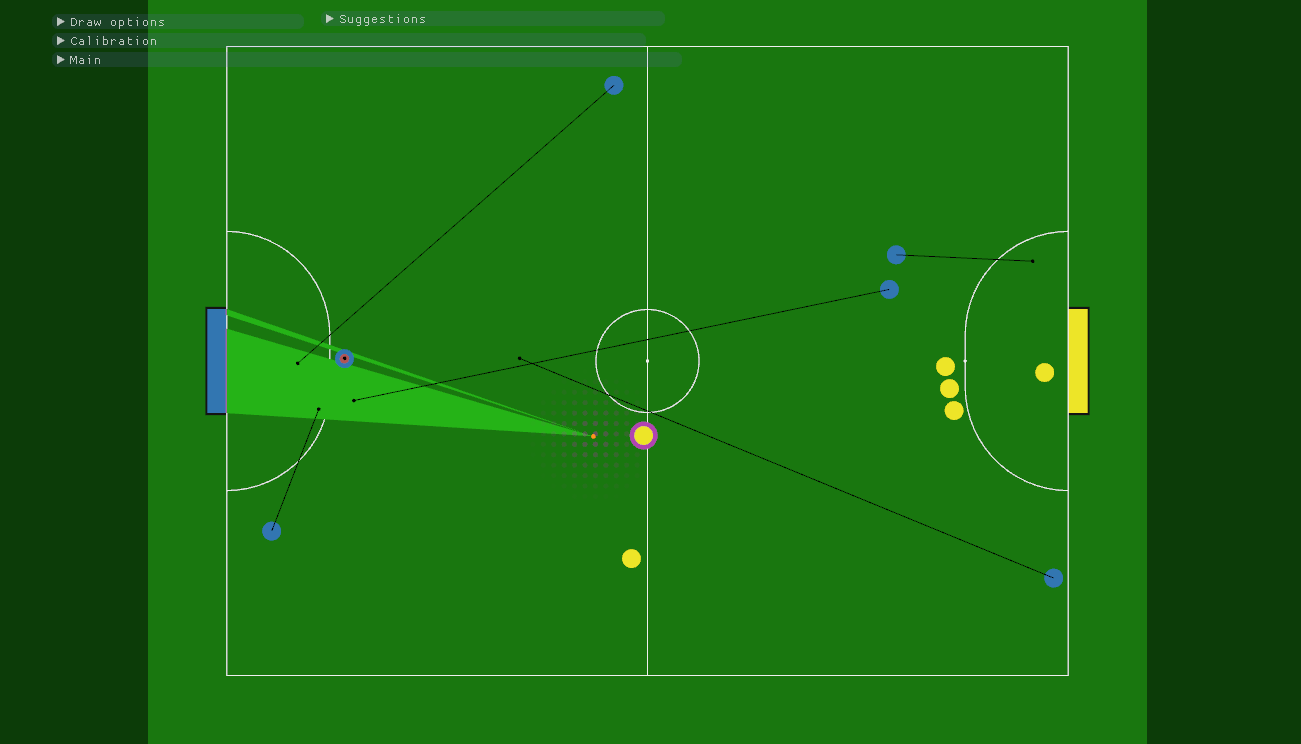
\includegraphics[width= 0.8\linewidth]{result/mov_dist_max_def_10}
  \caption{Planejamento com os parâmetros iniciais e o peso do
           custo da distância máxima dos moves alterado para $10$.
           Ataque (acima) e na defesa (abaixo)}\label{fig:mov_dist_max_10}
\end{figure}

\subsection{Custo do Ataque}
Somente o peso do custo do ataque foi alterado para $5000$.
Os resultados no planejamento são apresentados na
figura~\ref{fig:atack_5000}.

\begin{figure}[H]
  \centering
  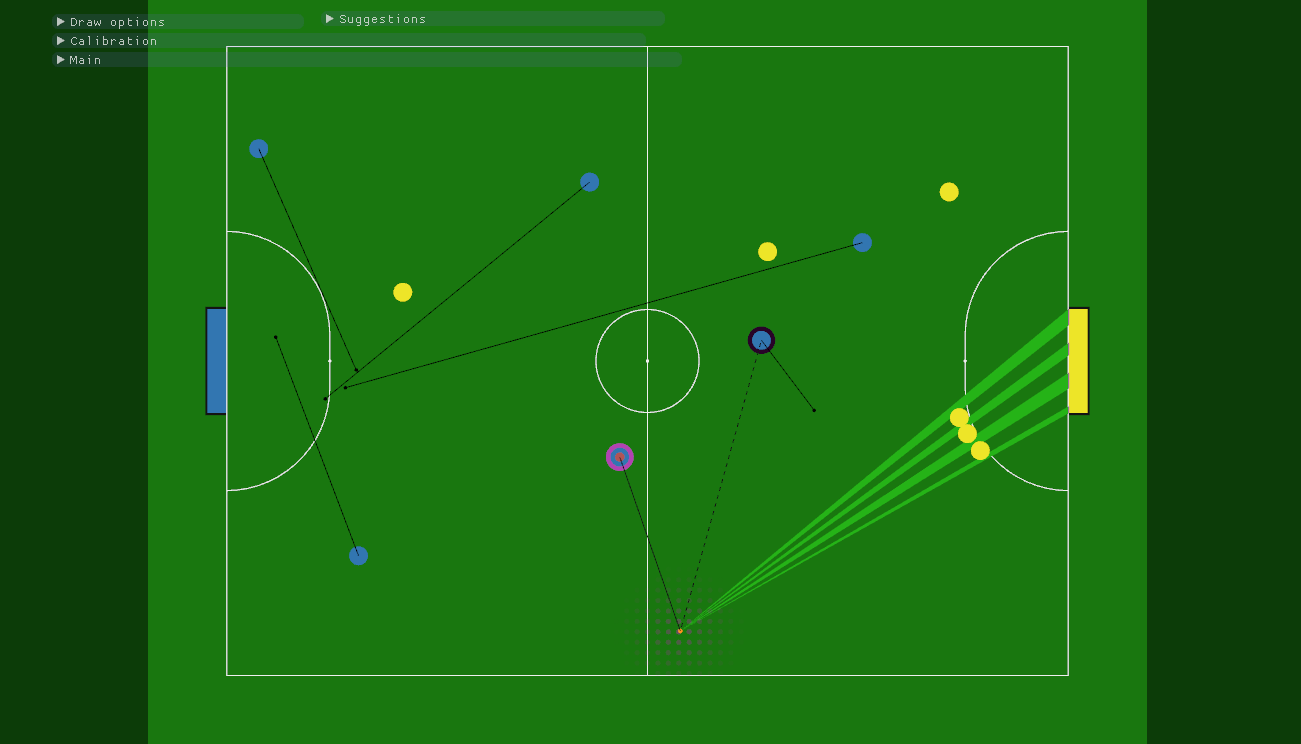
\includegraphics[width= 0.8\linewidth]{result/atack_atq_5000}
  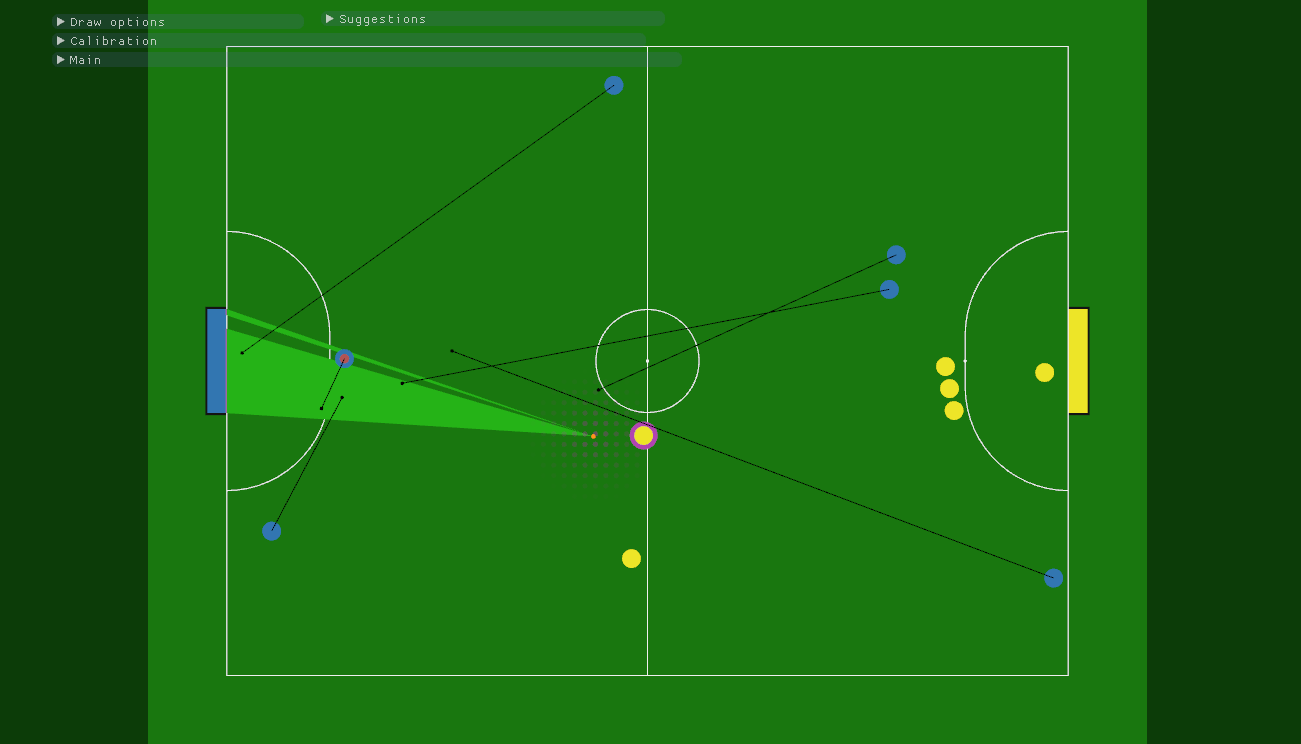
\includegraphics[width= 0.8\linewidth]{result/atack_def_5000}
  \caption{Planejamento com os parâmetros iniciais e o peso do
           custo do ataque alterado para $5000$.
           No ataque (acima) e na defesa (abaixo)}\label{fig:atack_5000}
\end{figure}

\subsection{Custo das Aberturas vistas por $r \in T_c$}

Somente o peso do custo das aberturas do gol vistas pelos robôs do time foi
alterado para $1000$. Os resultados no planejamento são apresentados na
Figura~\ref{fig:see_enemy_goal_1000}. Fica evidente em ambos os ambientes de
ataque e defesa que os robôs se posicionaram o mais próximo possível do gol de
$T_{ad}$, se limitando apenas pela penalização por proximidade do gol
adversário.

\begin{figure}[H]
  \centering
  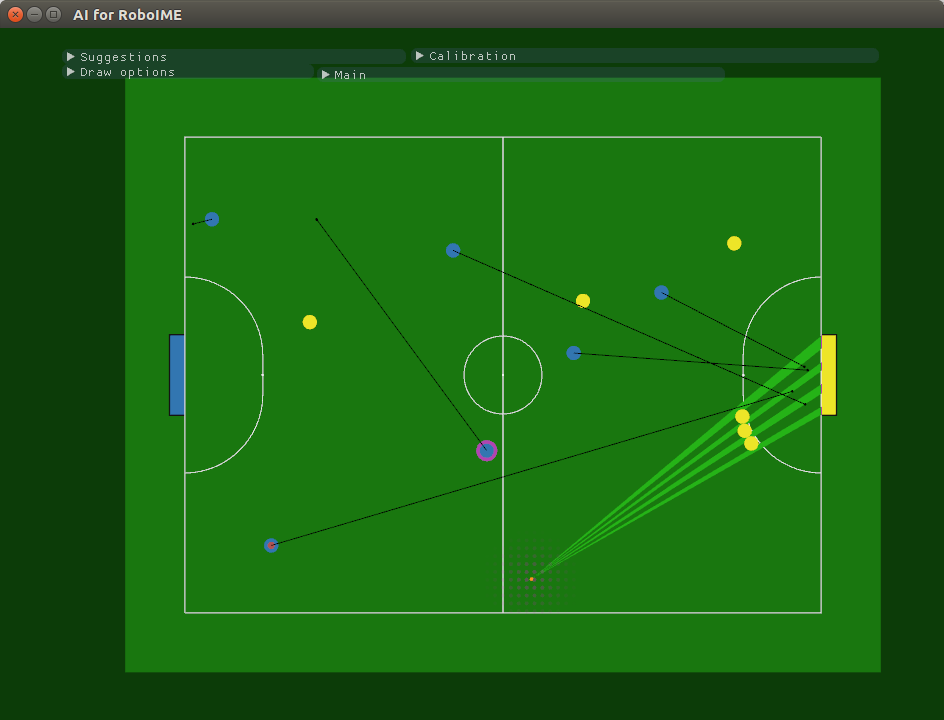
\includegraphics[width= 0.8\linewidth]{result/see_enemy_goal_atq_1000}
  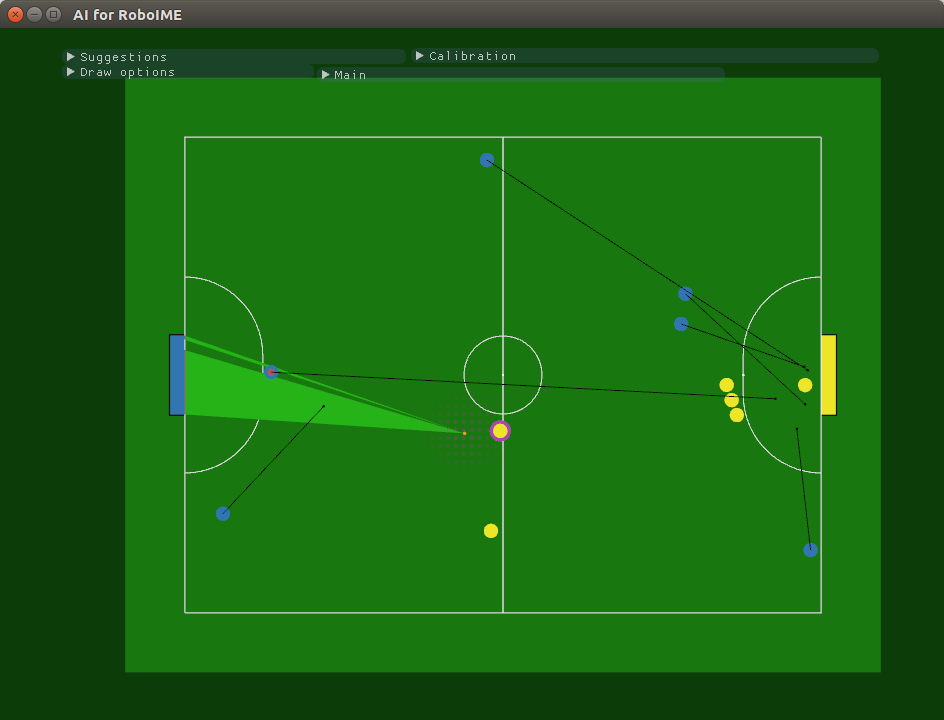
\includegraphics[width= 0.8\linewidth]{result/see_enemy_goal_def_1000}
  \caption{Planejamento com os parâmetros iniciais e com o peso do custo das
  aberturas do gol vistas pelos robôs do time igual a $1000$.  No ataque (acima)
  e na defesa (abaixo)}\label{fig:see_enemy_goal_1000}
\end{figure}

% vim: tw=80 et ts=2 sw=2 sts=2 ft=tex

\subsection{Custo das Aberturas vistas por $r \in T_{ad}$}
Somente o peso do custo das aberturas do goal vistas pelos robôs do time
adversário alterado para zero. Os resultados no planejamento são
apresentados na Figura~\ref{fig:block_goal_0}. Houve uma redução nas
posições de defesa com e sem posse de bola.

\begin{figure}[H]
  \centering
  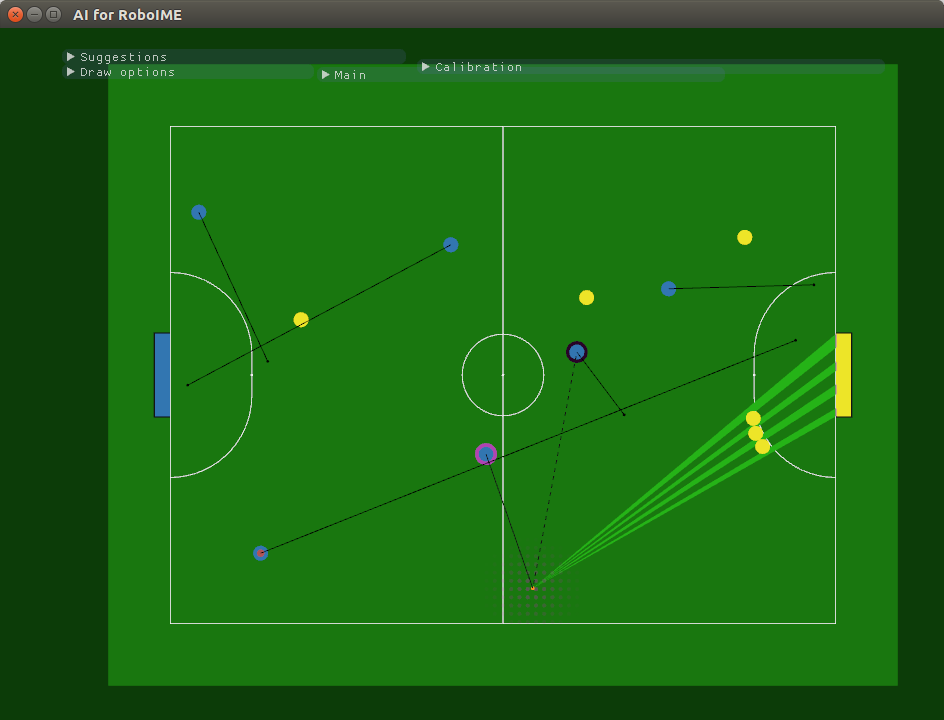
\includegraphics[width= 0.8\linewidth]{result/block_goal_atq_0}
  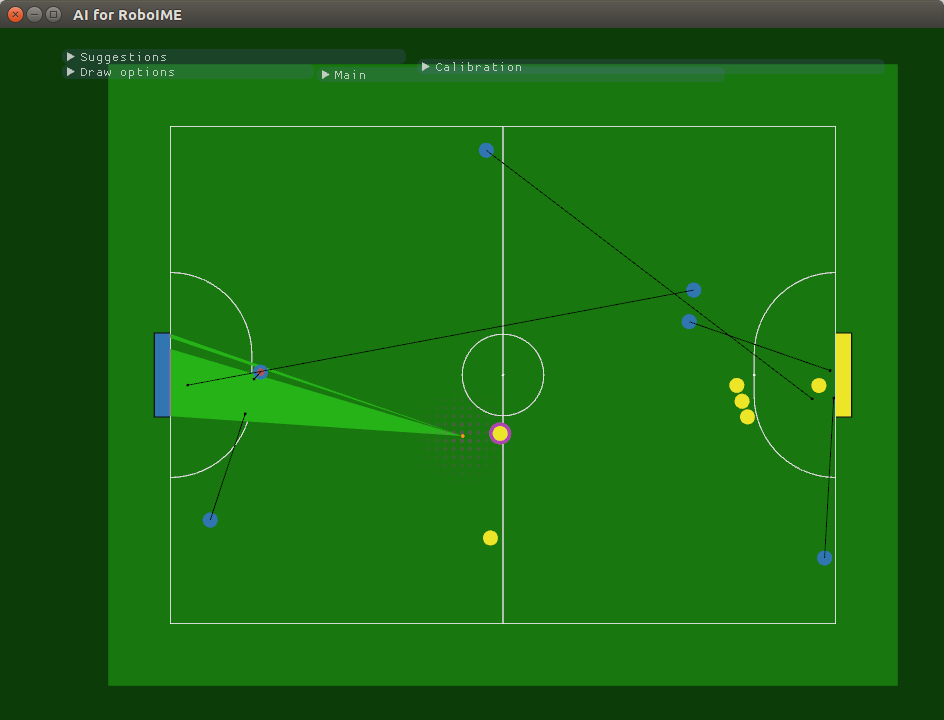
\includegraphics[width= 0.8\linewidth]{result/block_goal_def_0}
  \caption{Planejamento com os parâmetros iniciais e com o custo
           das aberturas do goal vistos pelos robôs do time nulo.
           No ataque (acima) e na defesa (abaixo)}\label{fig:block_goal_0}
\end{figure}

\subsection{Abertura mínima para chute a gol}

Somente o peso do parâmetro que permite chute a gol foi alterado para $5$.  Os
resultados no planejamento são apresentados na Figura~\ref{fig:min_gap_5}.
Conforme pode ser visto, somente no ambiente de ataque houve uma mudança grande,
gerando uma ação de chute no lugar de uma ação de passe.

\begin{figure}[H]
  \centering
  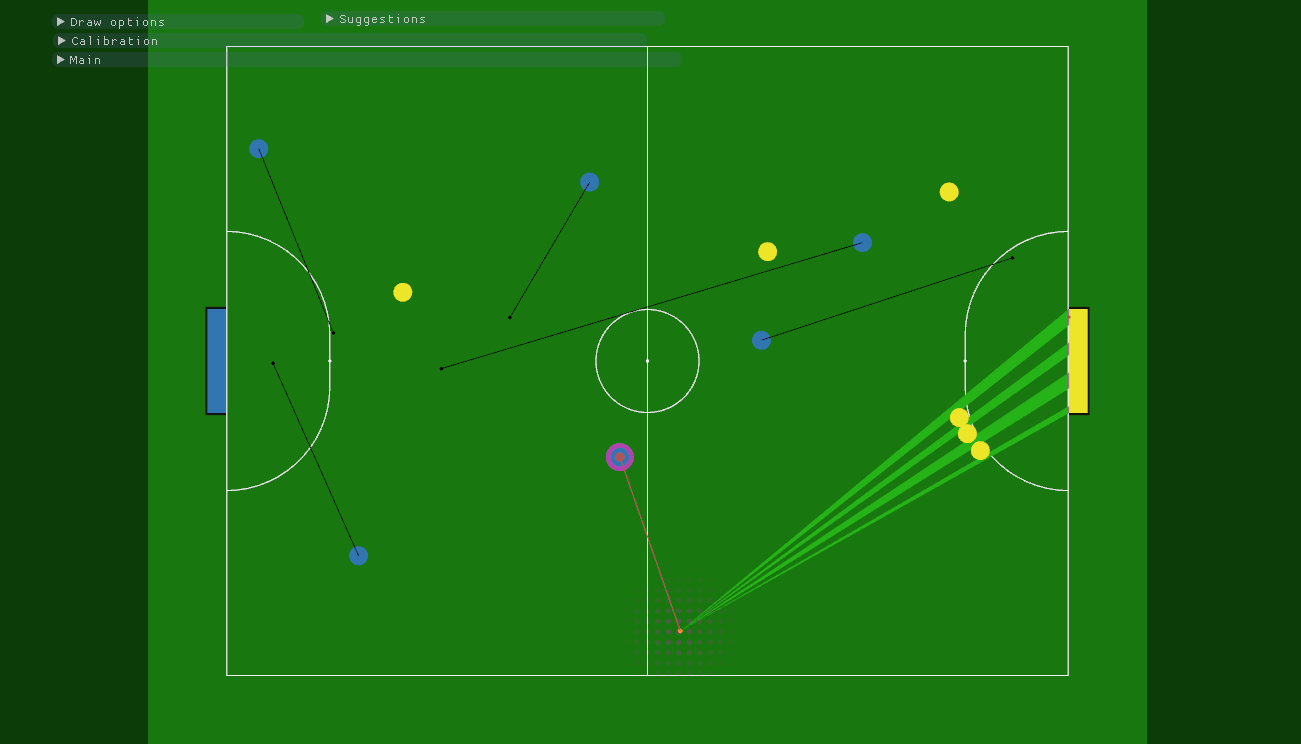
\includegraphics[width= 0.8\linewidth]{result/min_gap_atq_5}
  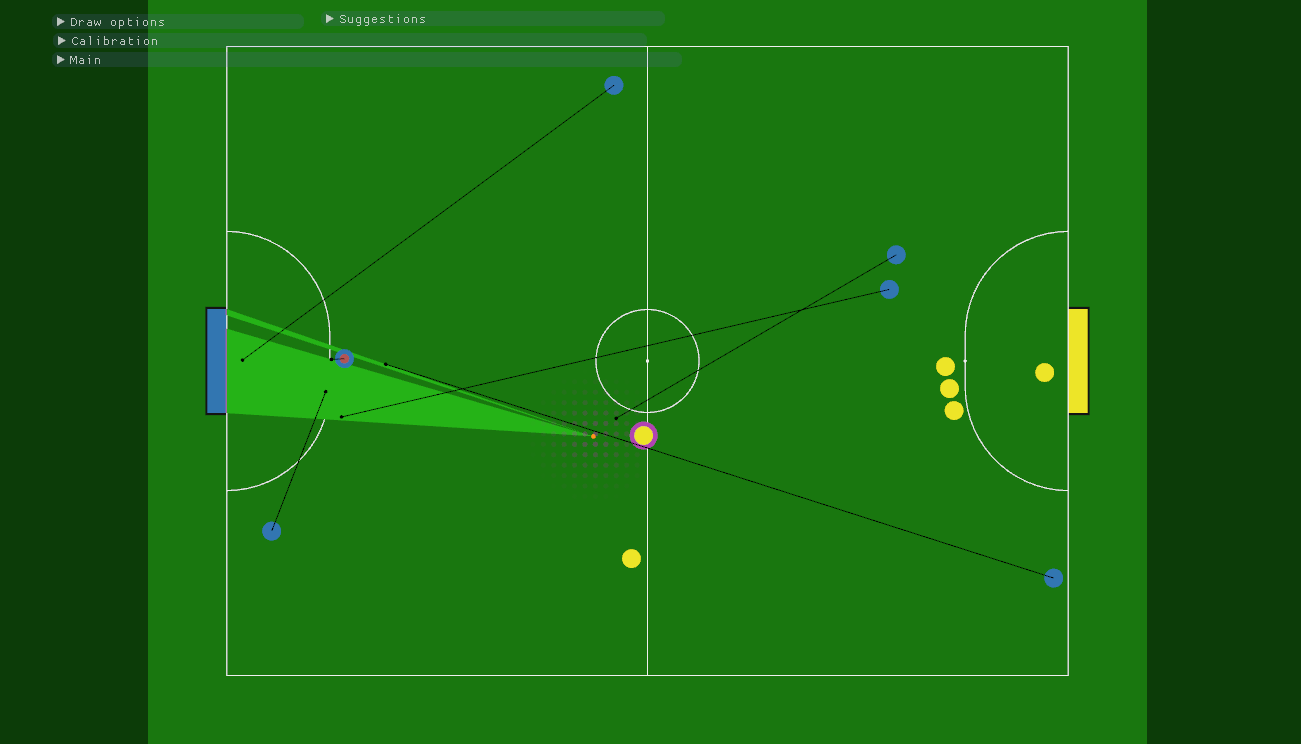
\includegraphics[width= 0.8\linewidth]{result/min_gap_def_5}
  \caption{Planejamento com os parâmetros iniciais e com a abertura mínima para
  chute alterado para $5$.  No ataque (acima) e na defesa (abaixo)}\label{fig:min_gap_5}
\end{figure}

% vim: tw=80 et ts=2 sw=2 sts=2 ft=tex spelllang=pt_br,en


% vim: tw=80 et ts=2 sw=2 sts=2 ft=tex
